%%%%%%%%%%%%%%%%%%%%%%%%%%%%%%%%%%%%%%%%%
% Programming/Coding Assignment
% LaTeX Template
%
% This template has been downloaded from:
% http://www.latextemplates.com
%
% Original author:
% Ted Pavlic (http://www.tedpavlic.com)
%
% Note:
% The \lipsum[#] commands throughout this template generate dummy text
% to fill the template out. These commands should all be removed when
% writing assignment content.
%
% This template uses a Python script as an example snippet of code, most other
% languages are also usable. Configure them in the "CODE INCLUSION
% CONFIGURATION" section.
%
%%%%%%%%%%%%%%%%%%%%%%%%%%%%%%%%%%%%%%%%%

%----------------------------------------------------------------------------------------
%	PACKAGES AND OTHER DOCUMENT CONFIGURATIONS
%----------------------------------------------------------------------------------------

\documentclass{article}

\usepackage{fancyhdr} % Required for custom headers
\usepackage{lastpage} % Required to determine the last page for the footer
\usepackage{extramarks} % Required for headers and footers
\usepackage[usenames,dvipsnames]{color} % Required for custom colors
\usepackage{graphicx} % Required to insert images
\usepackage{listings} % Required for insertion of code
\usepackage{courier} % Required for the courier font
\usepackage{lipsum} % Used for inserting dummy 'Lorem ipsum' text into the template
\usepackage{authblk}
\usepackage{amsmath}
\usepackage{placeins}
\usepackage{subfig}
\usepackage{tabularx}




% Margins
\topmargin=-0.45in
\evensidemargin=0in
\oddsidemargin=0in
\textwidth=6.5in
\textheight=9.0in
\headsep=0.25in

\linespread{1.1} % Line spacing

% Set up the header and footer
\pagestyle{fancy}
\lhead{\hmwkAuthorName} % Top left header
\rhead{\firstxmark} % Top right header
\lfoot{\lastxmark} % Bottom left footer
\cfoot{} % Bottom center footer
\rfoot{Page\ \thepage\ of\ \protect\pageref{LastPage}} % Bottom right footer
\renewcommand\headrulewidth{0.4pt} % Size of the header rule
\renewcommand\footrulewidth{0.4pt} % Size of the footer rule

\setlength\parindent{0pt} % Removes all indentation from paragraphs

%----------------------------------------------------------------------------------------
%	CODE INCLUSION CONFIGURATION
%----------------------------------------------------------------------------------------

\definecolor{MyDarkGreen}{rgb}{0.0,0.4,0.0} % This is the color used for comments
\lstloadlanguages{Python} % Load Python syntax for listings, for a list of other languages supported see: ftp://ftp.tex.ac.uk/tex-archive/macros/latex/contrib/listings/listings.pdf
\lstset{language=Python, % Use Python in this example
        frame=single, % Single frame around code
        basicstyle=\small\ttfamily, % Use small true type font
        keywordstyle=[1]\color{Blue}\bf, % Python functions bold and blue
        keywordstyle=[2]\color{Purple}, % Python function arguments purple
        keywordstyle=[3]\color{Blue}\underbar, % Custom functions underlined and blue
        identifierstyle=, % Nothing special about identifiers
        commentstyle=\usefont{T1}{pcr}{m}{sl}\color{MyDarkGreen}\small, % Comments small dark green courier font
        stringstyle=\color{Purple}, % Strings are purple
        showstringspaces=false, % Don't put marks in string spaces
        tabsize=5, % 5 spaces per tab
        %
        % Put standard Python functions not included in the default language here
        morekeywords={rand},
        %
        % Put Python function parameters here
        morekeywords=[2]{on, off, interp},
        %
        % Put user defined functions here
        morekeywords=[3]{test},
       	%
        morecomment=[l][\color{Blue}]{...}, % Line continuation (...) like blue comment
        numbers=left, % Line numbers on left
        firstnumber=1, % Line numbers start with line 1
        numberstyle=\tiny\color{Blue}, % Line numbers are blue and small
        stepnumber=5 % Line numbers go in steps of 5
}

% Creates a new command to include a Python script, the first parameter is the filename of the script (without .py), the second parameter is the caption
\newcommand{\Pythonscript}[2]{
\begin{itemize}
\item[]\lstinputlisting[caption=#2,label=#1]{#1.py}
\end{itemize}
}

%----------------------------------------------------------------------------------------
%	DOCUMENT STRUCTURE COMMANDS
%	Skip this unless you know what you're doing
%----------------------------------------------------------------------------------------

% Header and footer for when a page split occurs within a problem environment
\newcommand{\enterProblemHeader}[1]{
\nobreak\extramarks{#1}{#1 continued on next page\ldots}\nobreak
\nobreak\extramarks{#1 (continued)}{#1 continued on next page\ldots}\nobreak
}

% Header and footer for when a page split occurs between problem environments
\newcommand{\exitProblemHeader}[1]{
\nobreak\extramarks{#1 (continued)}{#1 continued on next page\ldots}\nobreak
\nobreak\extramarks{#1}{}\nobreak
}

\setcounter{secnumdepth}{0} % Removes default section numbers
\newcounter{homeworkProblemCounter} % Creates a counter to keep track of the number of problems

\newcommand{\homeworkProblemName}{}
\newenvironment{homeworkProblem}[1][Problem \arabic{homeworkProblemCounter}]{ % Makes a new environment called homeworkProblem which takes 1 argument (custom name) but the default is "Problem #"
\stepcounter{homeworkProblemCounter} % Increase counter for number of problems
\renewcommand{\homeworkProblemName}{#1} % Assign \homeworkProblemName the name of the problem
\section{\homeworkProblemName} % Make a section in the document with the custom problem count
\enterProblemHeader{\homeworkProblemName} % Header and footer within the environment
}{
\exitProblemHeader{\homeworkProblemName} % Header and footer after the environment
}

\newcommand{\problemAnswer}[1]{ % Defines the problem answer command with the content as the only argument
\noindent\framebox[\columnwidth][c]{\begin{minipage}{0.98\columnwidth}#1\end{minipage}} % Makes the box around the problem answer and puts the content inside
}

\newcommand{\homeworkSectionName}{}
\newenvironment{homeworkSection}[1]{ % New environment for sections within homework problems, takes 1 argument - the name of the section
\renewcommand{\homeworkSectionName}{#1} % Assign \homeworkSectionName to the name of the section from the environment argument
\subsection{\homeworkSectionName} % Make a subsection with the custom name of the subsection
\enterProblemHeader{\homeworkProblemName\ [\homeworkSectionName]} % Header and footer within the environment
}{
\enterProblemHeader{\homeworkProblemName} % Header and footer after the environment
}

%----------------------------------------------------------------------------------------
%	NAME AND CLASS SECTION
%----------------------------------------------------------------------------------------

\newcommand{\hmwkTitle}{Homework\ \#2} % Assignment title
\newcommand{\hmwkDueDate}{Wednesday,\ September\ 27,\ 2017} % Due date
\newcommand{\hmwkClass}{CS\ 5727} % Course/class
\newcommand{\hmwkAuthorName}{Zhan Zhang and Jialiang Wang} % Your name
\newcommand{\netid}{zz524 and jw2476} % Your name

%----------------------------------------------------------------------------------------
%	TITLE PAGE
%----------------------------------------------------------------------------------------
\author{
  Zhan Zhang\\
  \texttt{zz524@cornell.edu}
  \and
  Jialiang Wang\\
  \texttt{jw2476@cornell.edu}
}
\title{
\vspace{2in}
\textmd{\textbf{\hmwkClass:\ \hmwkTitle}}\\
\normalsize\vspace{0.1in}\small{Due\ on\ \hmwkDueDate}\\
\vspace{3in}
}



%----------------------------------------------------------------------------------------

\begin{document}
\maketitle

%----------------------------------------------------------------------------------------
%	TABLE OF CONTENTS
%----------------------------------------------------------------------------------------

%\setcounter{tocdepth}{1} % Uncomment this line if you don't want subsections listed in the ToC

\newpage
\tableofcontents
\newpage

%----------------------------------------------------------------------------------------
%	PROBLEM 1
%----------------------------------------------------------------------------------------

% To have just one problem per page, simply put a \clearpage after each problem
\section{PROGRAMMING EXERCISES}
\begin{homeworkProblem}
(b) A sample face image is displayed in figure \ref{faceImg}.\\
  \begin{figure}
    \centering
    
\includegraphics[width=3cm]{pic/person01_01.png}
    \caption{Sample Face Image}
    \label{faceImg}
  \end{figure}

(c) The average face is displayed in figure \ref{aveFace}.\\
  \begin{figure}
    \centering
    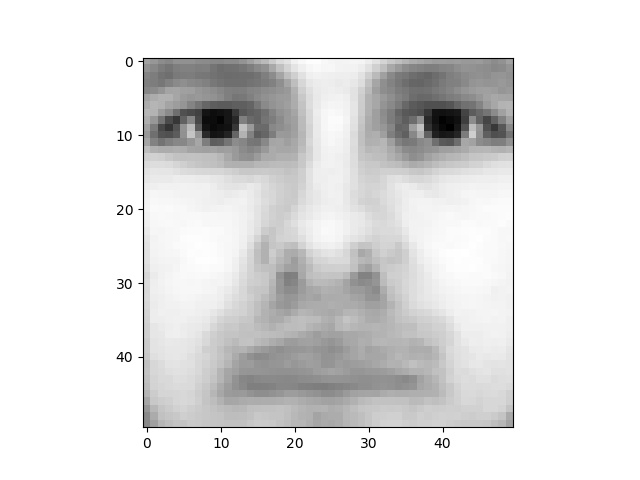
\includegraphics[width=3cm]{pic/mean_train}
    \caption{Average Face Image from the Training Set}
    \label{aveFace}
  \end{figure}

(d) A mean subtraction from the training set is display in figure \ref{meanSub} (a).\\
  \begin{figure}
    \centering
    \begin{tabular}{cc}
         \subfloat[Eigenface 1]{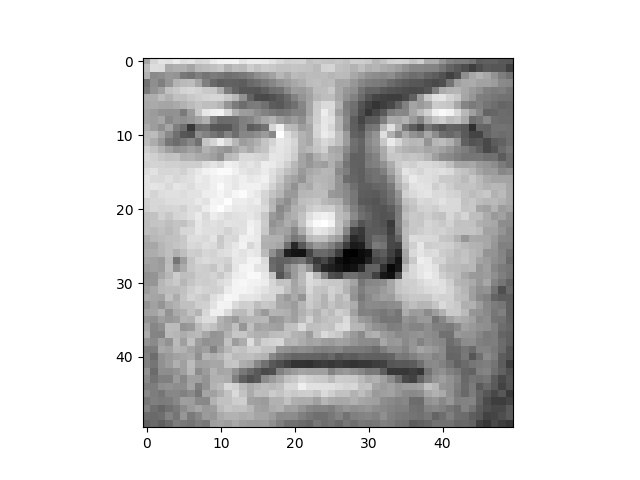
\includegraphics[width=3cm]{pic/mean_subtraction_train}}
       & \subfloat[Eigenface 2]{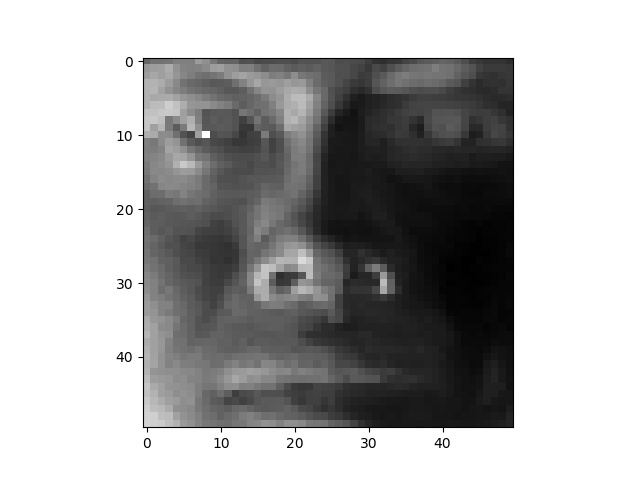
\includegraphics[width=3cm]{pic/mean_subtraction_test}}
     \end{tabular}
    \caption{Mean Subtraction Face Images}
    \label{meanSub}
  \end{figure}
A mean subtraction from the testing set is display in figure \ref{meanSub} (b).\\

(e) The first 10 eigenfaces are displayed in figure \ref{eigFace}.\\
  \begin{figure}
    \begin{tabular}{ccccc}
         \subfloat[Eigenface 1]{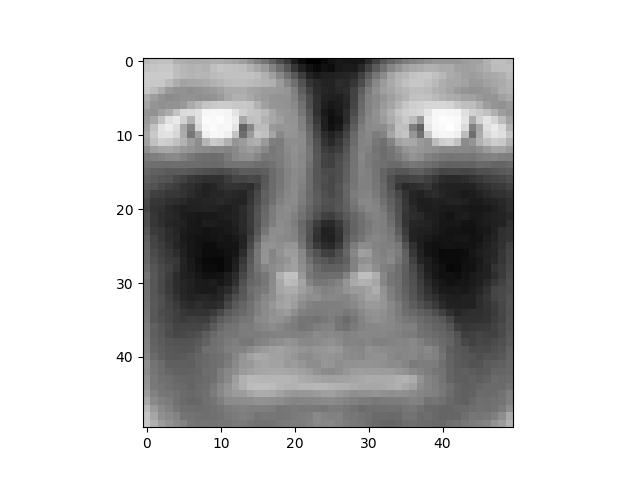
\includegraphics[width=3cm]{pic/svd_0_}}
       & \subfloat[Eigenface 2]{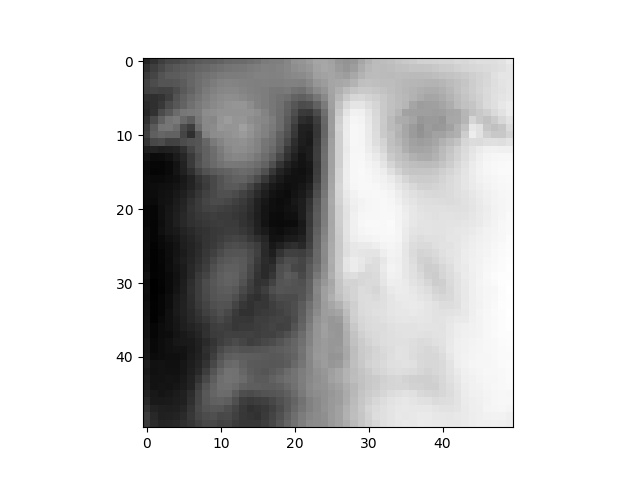
\includegraphics[width=3cm]{pic/svd_1_}}
       & \subfloat[Eigenface 3]{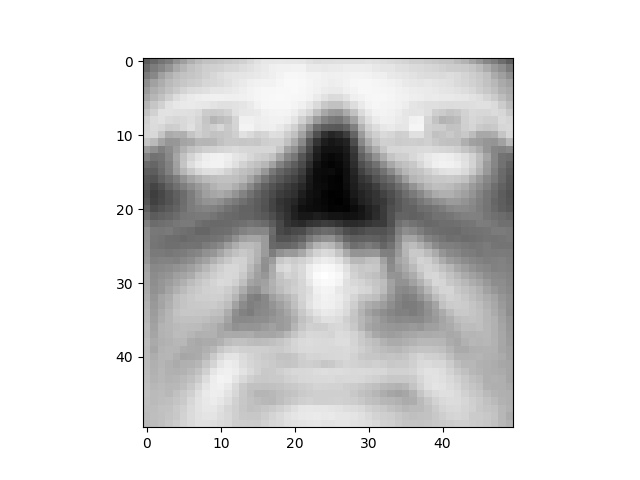
\includegraphics[width=3cm]{pic/svd_2_}}
       & \subfloat[Eigenface 4]{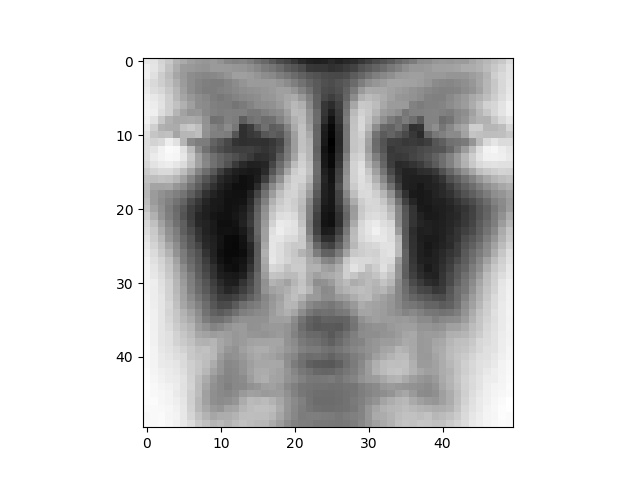
\includegraphics[width=3cm]{pic/svd_3_}}
       & \subfloat[Eigenface 5]{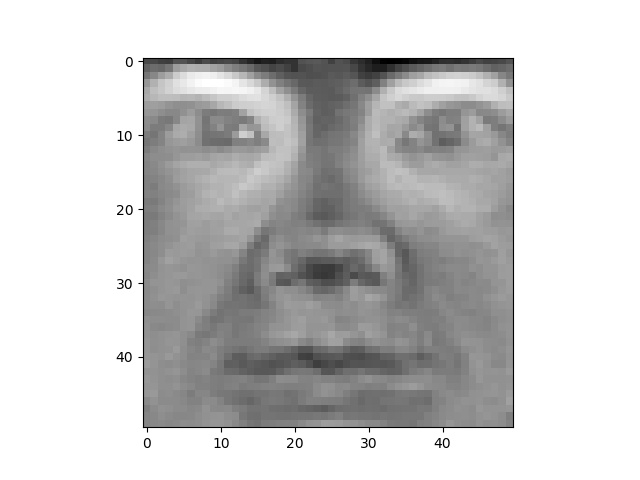
\includegraphics[width=3cm]{pic/svd_4_}}\\
        \subfloat[Eigenface 6]{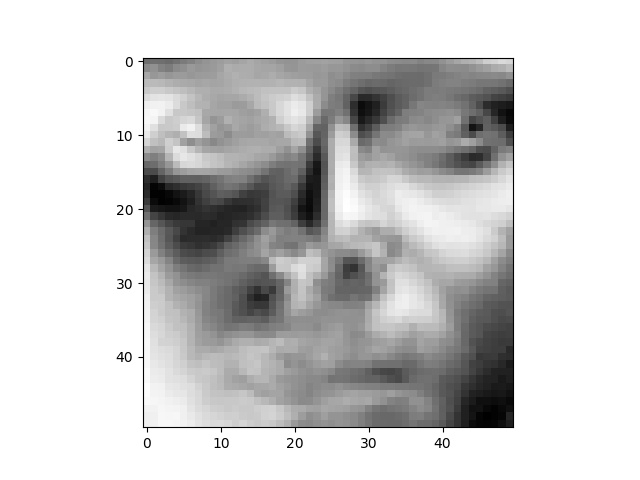
\includegraphics[width=3cm]{pic/svd_5_}}
       & \subfloat[Eigenface 7]{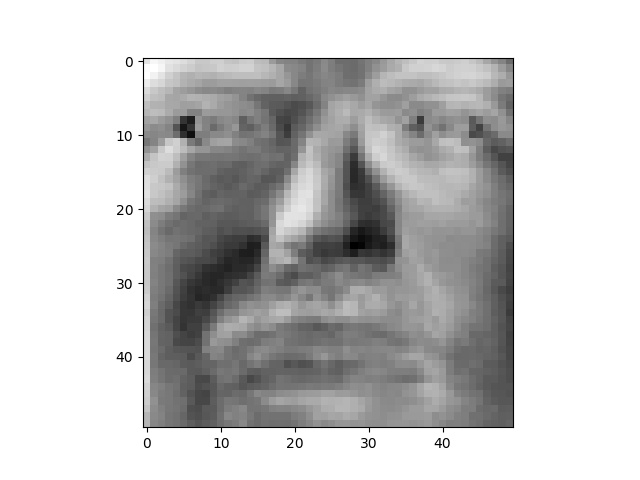
\includegraphics[width=3cm]{pic/svd_6_}}
       & \subfloat[Eigenface 8]{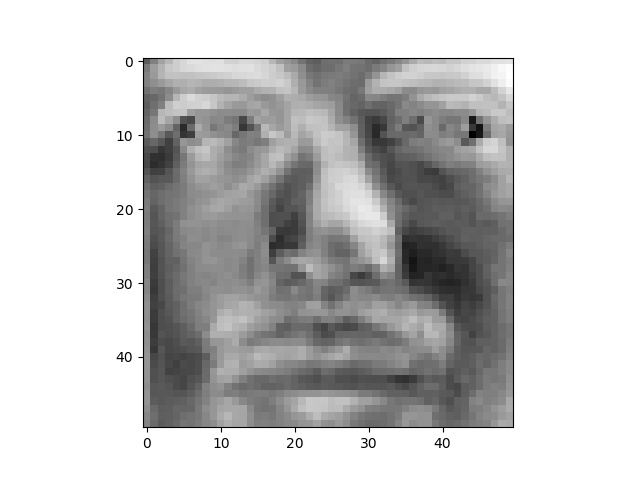
\includegraphics[width=3cm]{pic/svd_7_}}
       & \subfloat[Eigenface 9]{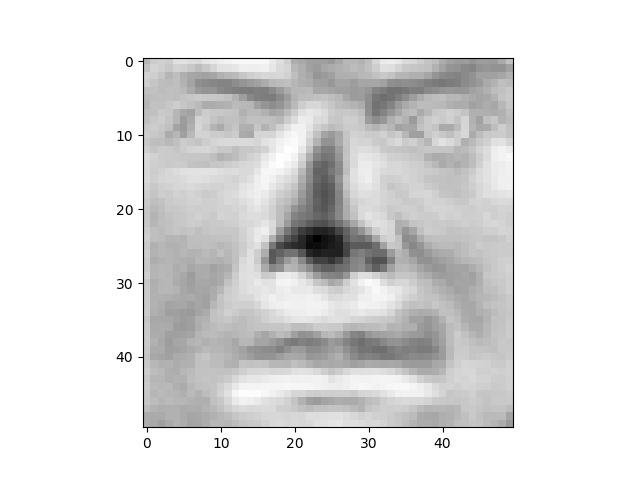
\includegraphics[width=3cm]{pic/svd_8_}}
       & \subfloat[Eigenface 10]{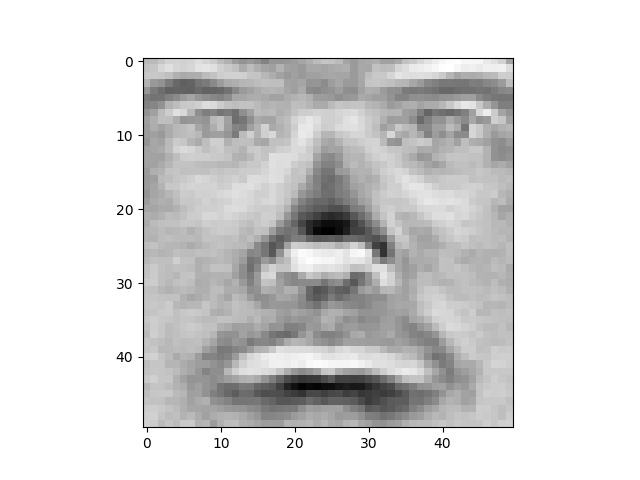
\includegraphics[width=3cm]{pic/svd_9_}}\\
    \end{tabular}
  \caption{Eigenfaces}
  \label{eigFace}
  \end{figure}

(f) The plot for the rank-r approximation error is shown in figure \ref{approximation}.\\
  \begin{figure}
    \centering
    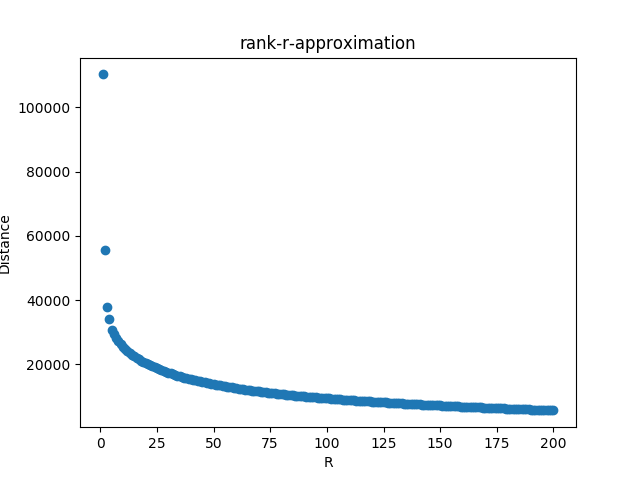
\includegraphics[width=0.8\textwidth]{pic/approximation}
    \caption{Rank-r Approximation Error}
    \label{approximation}
  \end{figure}

(h) The classification accuracy from the logistic model trained is plotted in figure \ref{accurlog}.\\
\begin{figure}
  \centering
  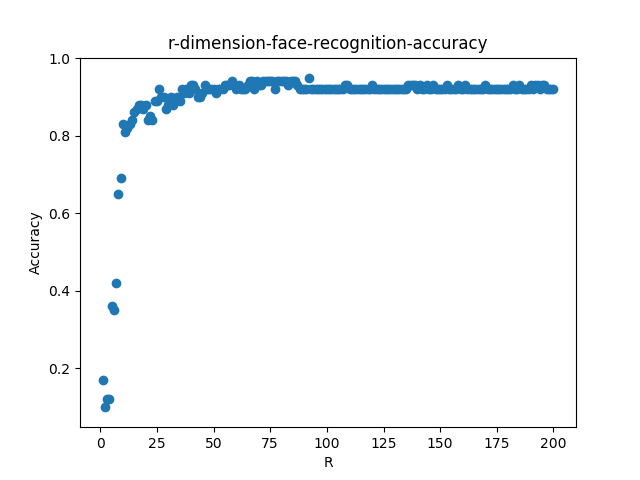
\includegraphics[width=0.8\textwidth]{pic/logistic_face_accuracy}
  \caption{Classification Accuracy of the Logistic Model}
  \label{accurlog}
\end{figure}
\end{homeworkProblem}

\begin{homeworkProblem}
(b)\begin{itemize}
    \item There are 39774 samples in the training set;
    \item There are 20 categories in the training set;
    \item There are 6714 unique ingredients appearing in the training set;
    \item There are 7137 unique ingredients appearing in both the training and testing set.
  \end{itemize}
  (d) The average accuracy for 3-fold cross-validation for both Gaussian prior and Bernoulli
  prior are 0.38215893891 and 0.678408428328.\\
  System with Bernoulli prior have a performance much better than the one with Gaussian piror.\\
  This could be explained from that the features (ingredients) are mark as 0 or 1 (exists or non-exists)
  which is a better fit for the Bernoulli Distribution.\\
  (f) The average accuracy for 3-fold cross-validation for Logistic Regression is 0.775758670409.\\
  (g) The outcome has been submitted to kaggle, shown in figure \ref{cookingKaggle}.
  \begin{figure}
    \centering
    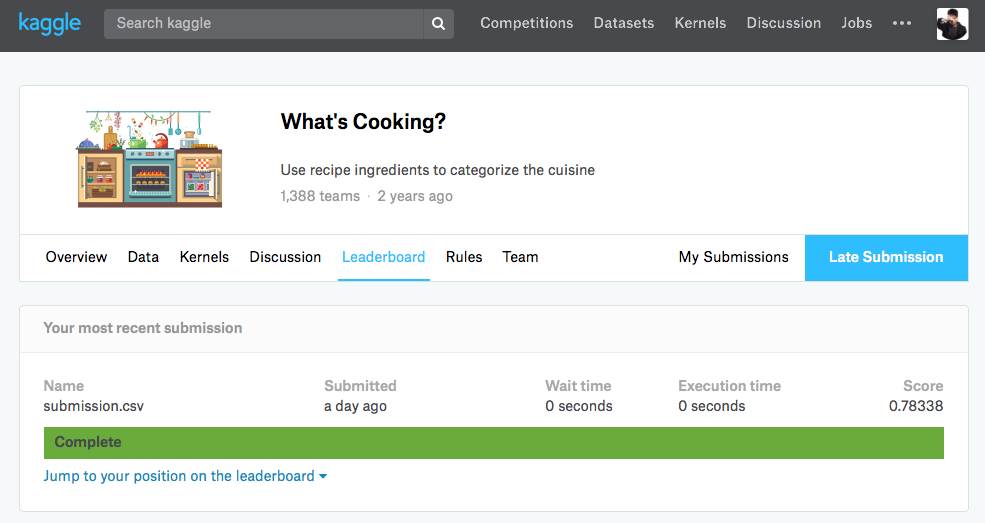
\includegraphics[width = 0.6\linewidth]{pic/kaggle2.png}
    \caption{Kaggle What's Cooking Submission Record}
    \label{cookingKaggle}
  \end{figure}
\end{homeworkProblem}

\section{WRITTEN EXERCISES}

\begin{homeworkProblem}
It subjects to Lagrange multiplier condition : $$d\mathcal{L} / da = a^TB^T + a^TB - \lambda (a^TW^T + a^TW) =a^T[ (B^T - \lambda W^T) + (B - \lambda W) ]=0 $$
 So this problem becomes $Ba = \lambda Wa$

 By Cholesky decomposition, $W = LDL^T = DD^T, B = DCD^T$
 so $$DCD^Ta = \lambda DD^Ta $$
 So that $C(D^Ta) = \lambda (D^Ta)$
 \\let $(D^Ta) = y$, then $$Cy = \lambda y$$
 In this way, we convert the problem of find x to maximize $a^TBa$ to compute a matrix C and find a y st. $$Cy = \lambda y$$ and $y = D^Ta$
\end{homeworkProblem}
\begin{homeworkProblem}
  Please see the handwritten appendix for the solution.
\end{homeworkProblem}
\begin{homeworkProblem}
(a)\begin{equation}
  M^{T}M =
  \begin{bmatrix}
    39 &	57 &	60\\
    57 &	118 &	53\\
    60 &	53 &	127
  \end{bmatrix}
\end{equation}
\begin{center}
  and
\end{center}
\begin{equation}
  MM^{T} =
  \begin{bmatrix}
    10&	9	&26	&3	&26\\
    9&	62&	8	&-5	&85\\
    26&	8	&72	&10	&50\\
    3&	-5&	10&	2	&-1\\
    26&	85&	50&	-1&	138
  \end{bmatrix}
\end{equation}\\

(b) The eigen values for both two matrices are 214.6705 and 69.3295.\\

(c) The eigen vectors for matrix $M_{T}M$ are the row vectors in the matrix:\\
\begin{equation}
  \begin{bmatrix}
    0.904534033733291&	0.0146040411173086&	0.426151268684285\\
    -0.301511344577764&	0.728597992755815&	0.615008840621910
  \end{bmatrix}
\end{equation}
The eigen vectors for matrix $MM_{T}$ are the row vectors in the matrix:
\begin{equation}
  \begin{bmatrix}
    0.143201385117688&	-0.944594949352975&	0.00448837927376996&	-0.244973232790239&	0.164929423163427\\
    0.525570082350403&	0.0470413984460477&	0.541872014065717& 0.453306436544331&	0.471647315618646
  \end{bmatrix}
\end{equation}

(d) The SVD for the original matrix M is:\\
\begin{equation}
  U =
  \begin{bmatrix}
    -0.164929423163427&	-0.244973232790239\\
    -0.471647315618646&	0.453306436544331\\
    -0.336470547433036&	-0.829439646984777\\
    -0.00330585055309077&	-0.169746590702150\\
    -0.798200311392409&	0.133106561666003
  \end{bmatrix}
\end{equation}
\begin{equation}
  \Sigma =
  \begin{bmatrix}
    14.6516377649769&	0\\
    0&	8.32643445923304
  \end{bmatrix}
\end{equation}
\begin{equation}
  X =
  \begin{bmatrix}
    -0.426151268684285&	0.0146040411173084&	-0.904534033733291\\
    -0.615008840621911&	0.728597992755815& 0.301511344577764
  \end{bmatrix}
\end{equation}

(e) The one-dimensional approximation to the matrix M is:
\begin{equation}
  M(recovered) =
  \begin{bmatrix}
    1.02978864496302&	-0.0352904633127328&	2.18579397826745\\
    2.94487812262642&	-0.100919847830279&	6.25069707133886\\
    2.10085952200109&	-0.0719956529420139&	4.45921220323874\\
    0.0206411160375204&	-0.000707363158274219&	0.0438121233519250\\
    4.98381429651495&	-0.170793411297470&	10.5784729045218
  \end{bmatrix}
\end{equation}
\end{homeworkProblem}
%----------------------------------------------------------------------------------------

\end{document}
